\chapter{Mercoledì 11/03/2020}
\section{Interrogazioni}
L'interrogazione è un'operazione di lettura che non modifica la base di dati. In certe circostanze un'interrogazione può coinvolgere più tabelle! Abbiamo due tipi di semantiche:
\begin{itemize}
	\item \textbf{dichiarativa}, in cui si esprimono le proprietà del risultato. Essa ricorre al \emph{calcolo relazionale} e consiste nell'effettiva semantica del linguaggio! Le interrogazioni sono espresse ad alto livello.
	\item \textbf{operazionale}, si specificano le modalità di calcolo adottate dal gestore della base di dati per ottenere il risultato. In questo caso si ricorre all'\emph{algebra relazionale}. Poichè si parla di modalità di calcolo possiamo individuare i costi per l'esecuzione di una certa interrogazione
\end{itemize}
\subsection{\emph{query processor}} All'interno del gestore abbiamo un modulo detto \emph{query processor}, dove è definito il processo di esecuzione delle interrogazioni. Ciò permette al gestore di definire una strategia di esecuzione ottimale. Si hanno tre fasi:
\begin{itemize}
	\item \textbf{Analisi lessicale, sintattica e semantica} della query scritta: si ottiene una corrispondente espressione algebrica;
	\item \textbf{Ottimizzazione algebrica} dell'espressione: si ottiene una nuova espressione algebrica attraverso ottimizzazioni valide in ogni caso (Esempio: \emph{push selections down} e \emph{push projections down})
	\item \textbf{Ottimizzazione basata sui costi}: sfruttando quanto contenuto nel cosiddetto \emph{catalogo}, cioè informazioni quantitative (\emph{profili}) riguardanti il database (numero di tuple, dimensione della tupla o dei valori, numero di valori distinti, valori minimi e massimi degli attributi...), possiamo stimare la dimensione dei risultati intermedi ed effettuare ulteriori ottimizzazioni (riparleremo di questa ottimizzazione nell'ultima lezione).
\end{itemize}

\subsubsection{Ottimizzazione algebrica}
Le due fasi di ottimizzazione si basano sull'euristica: sulla base dei dati a disposizione decidiamo quali procedure adottare per eseguire un'istruzione. Parlare di "euristica", tuttavia, è un po' improprio: il processo si basa soprattutto sulla nozione di equivalenza.
\paragraph{Equivalenza} Due espressioni sono equivalenti se producono lo stesso risultato!
\pagebreak

\section{Algebra relazionale}
Nell'algebra relazionale abbiamo operatori applicati su una o più relazioni. Gli operatori producono nuove relazioni e possono essere composti. Analizzeremo \textbf{operatori su insiemi} (unione, intersezione e differenza) ed \textbf{operatori su relazioni} (ridenominazione, selezione, proiezione, join). I primi operatori sono applicati a relazioni che presentano gli stessi attributi: la relazione prodotta avrà gli stessi attributi. I secondi, ad eccezione del join (il più complesso tra quelli che vedremo), sono monadici.\\

\noindent Nelle successive definizioni considereremo $X$ come l'insieme degli attributi.
\subsection{Unione ($r_1 \cup r_2$)}
Date due relazioni $r_1(X), r_2(X)$, l'unione $r_1(X) \cup r_2(X)$ consiste in una nuova relazione che contiene sia le tuple di $r_1$ che quelle di $r_2$.
\paragraph{Esempio dalle diapositive} Abbiamo le relazioni $\mathbf{laureati\_triennal}i$ e $\mathbf{laureati\_magistrali}$.\\
Ottengo una nuova relazione che elenca le persone che hanno conseguito almeno una laurea. Nei risultati della nuova relazione vediamo Neri e Verdi che hanno conseguito sia la laurea triennale che quella magistrale, un altro Neri che ha solo la laurea magistrale, Rossi che ha solo la laurea triennale.

\begin{center}
	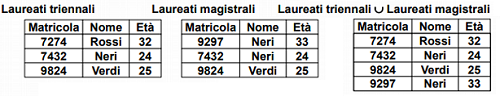
\includegraphics{images/28.PNG}
\end{center}

\subsection{Intersezione ($r_1 \cap r_2$)}
Date due relazioni $r_1(X), r_2(X)$, l'intersezione $r_1(X) \cap r_2(X)$ consiste in una nuova relazione che contiene solo le tuple appartenenti ad entrambe le relazioni.
\paragraph{Esempio dalle diapositive} Prendiamo lo stesso esempio di prima. Ottengo una nuova relazione che elenca le persone che hanno preso sia la laurea magistrale che quella triennale. Gli unici che hanno conseguito entrambe le lauree sono Neri e Verdi: nell'istanza avrò soltanto le loro tuple.
\begin{center}
	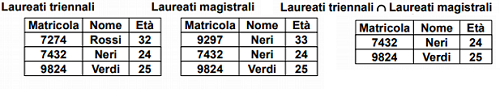
\includegraphics{images/29.PNG}
\end{center}
\pagebreak
\subsection{Differenza ($r_1 - r_2$)}
Date due relazioni $r_1(X), r_2(X)$, la differenza $r_1(X)-r_2(X)$ consiste in una nuova relazione che contiene le tuple di $r_1$ che non appartengono anche ad $r_2$. L'operatore è rappresentato dal segno meno.
\paragraph{Esempio dalle diapositive} Idem con patate. Ottengo una relazione in cui si hanno gli elementi di $\mathbf{laureati\_triennali}$ non presenti in $\mathbf{laureati\_magistrali}$, cioè coloro che hanno conseguito la laurea triennale ma non quella magistrale.\\Nella prima relazione abbiamo Rossi, Neri e Verdi: osserviamo che Neri e Verdi sono presenti anche nella seconda relazione. Segue che l'unica tupla presente nell'istanza sarà quella di Rossi.

\begin{center}
	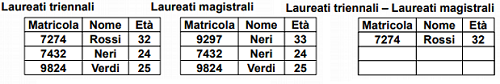
\includegraphics{images/30.PNG}
\end{center}

\subsection{Ridenominazione ($\rho_{a_1,\dots,a_n \leftarrow b_1,\dots,b_n}$)}
L'operatore monadico di ridenominazione ci permette di modificare lo schema di una relazione alterando gli attributi. Questa cosa ci permetterà di applicare gli operatori di insieme a relazioni che hanno schema simile ma non equivalente.
\paragraph{Esempio dalle diapositive} Abbiamo le relazioni $\mathbf{paternita}(padre,figlio)$ e $\mathbf{maternita}(madre,figlio)$ a cui voglio applicare l'operatore unione. Essi hanno schema simile, ma un attributo diverso. Mediante l'operatore di ridenominazione modifico l'attributo \emph{padre} in \emph{genitore}. Faccio la stessa cosa con \emph{madre}. A questo punto posso applico l'operatore di insieme.

\begin{center}
	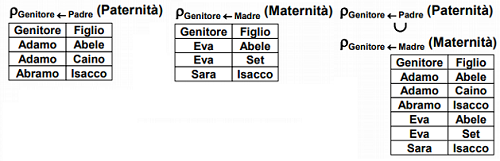
\includegraphics{images/31.PNG}
\end{center}

\subsection{Selezione ($\sigma_F$) - decomposizione orizzontale}
L'operatore monadico di selezione restituisce una nuova relazione con lo stesso schema ma con solo una parte delle tuple. Viene mostrato un sottoinsieme i cui elementi sono determinati a partire da un'espressione booleana $F$: se l'espressione è vera la tupla è considerata appartenente alla nuova relazione, altrimenti viene esclusa.
\paragraph{Esempio dalle diapositive} Ho una relazione $\mathbf{Impiegati}(matricola,cognome,filiale,stipendio,eta)$. Voglio mostrare soltanto gli impiegati con uno stipendio superiore ai 50.000 euro. Posso rendere la cosa più articolata mostrando soltanto gli impiegati che soddisfano la condizione precedente e che lavorano nella filiale di Milano.

\begin{center}
	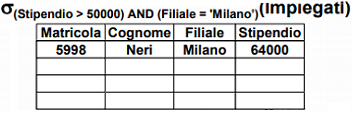
\includegraphics{images/32.PNG}
\end{center}

\paragraph{Attenzione ai valori nulli} Prendiamo la stessa relazione e consideriamo le persone con $eta > 40$. Le tuple con età nulla vengono automaticamente escluse: ciò può essere evitato indicando che il valore può essere anche nullo (Ho le forme \emph{IS NULL} e \emph{IS NOT NULL}). 
\[\sigma_{Eta > 40}(Impiegati)\;\;\;\;\;\sigma_{(Eta > 40)\, OR \;(Eta\; \mathbf{IS\;NULL})}(Impiegati)\]
\subsection{Proiezione ($\pi_Y$) - decomposizione verticale}
L'operatore monadico di proiezione restituisce una nuova relazione che contiene un insieme di tuple ristrette agli attributi Y (ho un sottoinsieme degli attributi, fondamentalmente).
\paragraph{Esempio dalle diapositive} Riprendiamo l'esempio utilizzato negli operatori di insieme: creo una nuova relazione in cui mostro soltanto matricole e cognomi.

\begin{center}
	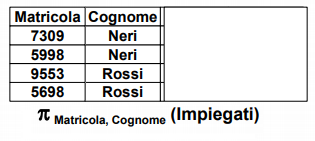
\includegraphics{images/33.PNG}
\end{center}

\paragraph{Cardinalità delle proiezioni} Può capitare che una proiezione produca una relazione con un numero inferiore di tuple. Ciò può avvenire escludendo la chiave \emph{matricola}. Osserviamo che sono presenti nella relazione iniziale due Neri e due Rossi. Nella relazione finale ho due Neri e un \emph{solo} Rossi poichè abbiamo ignorato l'attributo che identifica le tuple in modo univoco: si osserva, inoltre, che entrambi i Rossi lavorano nella filiale di Roma.

\begin{center}
	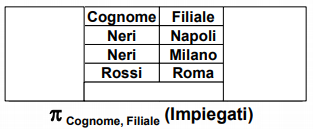
\includegraphics{images/34.PNG}
\end{center}

% Nelle due relazioni hanno la stessa età. Si osserva che nell'unione l'identità delle due relazioni viene persa e conseguentemente nella nuova relazione non si hanno duplicati: essa conterrà semplicemente le persone che si sono laureate almeno una volta.
\subsection{Composizione degli operatori}
Come già detto posso creare una composizione di operatori: per esempio posso unire l'operatore selezione con l'operatore proiezione. Nella composizione è necessario porre attenzione all'ordine degli operatori: un ordine diverso può portare a risultati diversi.

\begin{center}
	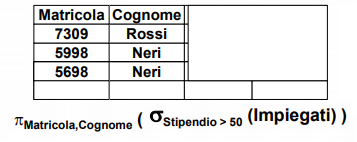
\includegraphics{images/35.PNG}
\end{center}
Adesso spingiamoci oltre: con gli operatori introdotti fino ad ora non possiamo correlare relazioni profondamente diverse tra loro!
\subsection{Operatore Join}
Con l'operatore JOIN ossiamo correlare dati appartenenti a relazione diverse!
\subsubsection{Prodotto cartesiano ($r_1 \times r_2$)}
Operatore binario, di fatto il più costoso per il DBMS. Abbiamo due relazioni: combiniamo le tuple di $r_1$ con le tuple di $r_2$. Ottengo una nuova relazione dove
\begin{itemize}
	\item lo schema consiste nell'unione degli attributi delle due relazioni
	\item l'istanza è caratterizzata da tuple ottenute mediante il prodotto cartesiano matematico.
\end{itemize}
\begin{center}
	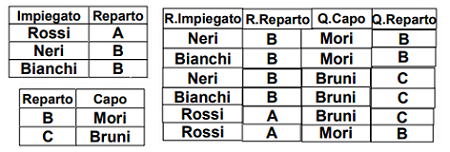
\includegraphics{images/38.PNG}
\end{center}
\subsubsection{Join naturale ($r_1 \Join r_2$)}
Il \emph{join naturale} è un operatore binario che restituisce una relazione con schema uguale all'unione degli attributi degli schemi di $r_1(X_1)$ e $r_2(X_2)$ ($X_1 \cup X_2$). Si individua che 
\[r_1 \Join r_2=\{t \in X_1 \cup X_2\;|\; t[X_1] \in r_1, t[X_2] \in r_2\}\]
Il join naturale consiste in un insieme di tuple da cui ottengo tuple appartenenti alla relazione $r_1$ se applico una proiezione limitata a $X_1$ e tuple appartenenti alla relazione $r_2$ se applico una proiezione limitata a $X_2$.
Abbiamo due situazioni:
\begin{itemize}
	\item \textbf{presenza di attributi con lo stesso nome}: le tuple vengono costituite se il valore degli attributi comuni è uguale
	\item \textbf{senza attributi con nome comune}: quello che si ottiene equivale al prodotto cartesiano. Ho un numero di tuple pari al prodotto delle cardinalità degli operandi (le tuple sono tutte combinabili)
\end{itemize}
\paragraph{Osservazione} Solitamente non è possibile tornare alle relazioni originali dopo aver applicato il join.
\paragraph{Esempio dalle diapositive} Riprendiamo le relazioni $impiegati$ e $caporeparti$. Rossi non è tra le tuple poichè non è combinabile con nessun capo reparto. Si osserva che il capo del reparto C non può essere combinato con nessun impiegato (non si hanno impiegati al reparto C). 
\begin{center}
	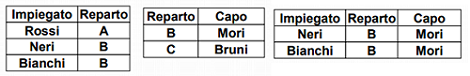
\includegraphics{images/36.PNG}
\end{center}
Potrebbe succedere che per un reparto (il B in questo caso) si abbiano due capireparto: Neri e Bianchi (del reparto B) vengono combinati due volte!
\begin{center}
	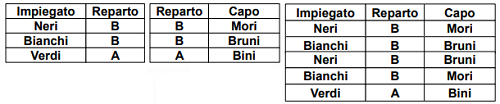
\includegraphics{images/37.PNG}
\end{center}
\paragraph{Esempio senza attributi comuni}
\begin{center}
	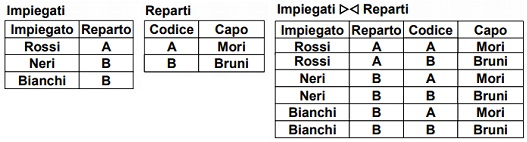
\includegraphics{images/39.PNG}
\end{center}
\paragraph{In generale}
\begin{itemize}
	\item Date due relazioni $R_1(X_1),R_2(X_2)$ si osserva che la proiezione di $X_1$ del join naturale tra $R_1$ e $R_2$ è inclusa in $R_1$.
	\[\pi_{X_1}(R_1\Join R_2) \subseteq R_1\]
	Se non si hanno attributi comuni avviene il prodotto cartesiano e il risultato dell'espressione coincide con $R_1$. Se si hanno attributi comuni il risultato non coincide con il prodotto cartesiano e due tuple vengono associate solo se si hanno le condizioni. Segue che il non-JOIN di alcune tabelle potrebbe comportarmi l'esclusione di alcune tuple di $R_1$ e quindi avere come risultato un sottoinsieme di $R_1$.
	\item Data una relazione $R(X)$, dove $X=X_1 \cup X_2$, il join naturale tra la proiezione di $X_1$ di $R$ e la proiezione di $X_2$ di $R$ contiene $R$
	\[(\pi_{X_1}(R))\Join(\pi_{X_2}(R))\supseteq R\]
	Se non si hanno attributi comuni tra $X_1$ e $X_2$ segue un prodotto cartesiano che mi porta ad avere un numero di tuple maggiore rispetto a prima. Ho quindi un insieme più grande che contiene l'insieme $R$ iniziale. Se ho attributi comuni tra $X_1$ e $X_2$ allora può esserci la possibilità che il risultato sia uguale ad $R$ originario.
\end{itemize}
\subsubsection{\emph{theta-join} (spesso \emph{equi-join})}
Posso ridurre il prodotto cartesiano attraverso una relazione del tipo $\sigma_F(R_1 \times R_2)$. La stessa operazione può essere fatta attraverso un operatore derivato detto \emph{theta-join}: prendo soltanto le tuple che fanno JOIN e che soddisfano delle condizioni.
\[R_1 \Join_F R_2\]
La condizione $F$ è spesso una congiunzioni di atomi di confronto caratterizzati da un operatore di confronto e attributi di relazioni diverse. Se l'operatore di confronto è l'uguale allora si ha l'\emph{equi-join}. \\
Riprendiamo l'esempio di prima dove non si hanno attributi comuni. Svolgiamo l'equi-join stabilendo un legame valido tra tuple se Reparto=Codice.
\begin{center}
	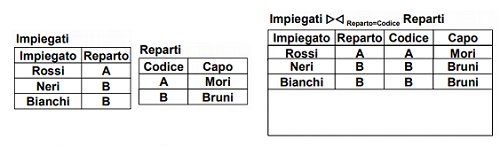
\includegraphics{images/40.PNG}
\end{center}
\subsection{JOIN operatore non primitivo}
\begin{center}
	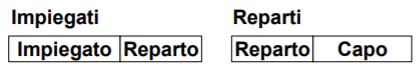
\includegraphics{images/75.PNG}
\end{center}
Il Join non è un operatore primitivo (diciamo, un "prodotto cartesiano schietto"). Individuiamo che
\paragraph{Relazione tra JOIN Naturale e prodotto cartesiano}
\[Impiegati \Join Reparti = \pi_{Impiegato,Reparto,Capo}(\sigma_{I.reparto=reparto}(\rho_{I.reparto \leftarrow Reparto}(Impiegati) \times Reparti))\]
\begin{itemize}
	\item Applico la ridenominazione alla relazione \emph{Impiegati} per poter usare la selezione
	\item Eseguo il prodotto cartesiano tra la relazione $\rho_{I.Reparto\leftarrow Reparto}(Impiegati)$ e \emph{Reparti}. 
	\item Applico la selezione, scegliendo i record che soddisfano la condizione $I.Reparto=Reparto$
	\item Proietto gli attributi $Impiegato, Reparto, Capo$. $I.Reparto$ ha lo stesso valore di $Reparto$, non serve proiettarlo nuovamente.
\end{itemize}
\paragraph{Relazione tra JOIN Naturale ed equi-join}
\[Impiegati \Join Reparti = \pi_{Impiegato,Reparto,Capo}(\rho_{I.reparto \leftarrow Reparto}(Impiegati) \Join_{I.Reparto=Reparto} Reparti)\]
\begin{itemize}
	\item Applico la ridenominazione alla relazione \emph{Impiegati} per poter usare la selezione
	\item Eseguo l'equi-JOIN tra la relazione $\rho_{I.Reparto\leftarrow Reparto}(Impiegati)$ e \emph{Reparti}, scegliendo soltanto le combinazioni di record che soddisfano l'uguaglianza $I.Reparto=Reparto$
	\item Proietto gli attributi $Impiegato, Reparto, Capo$. $I.Reparto$ ha lo stesso valore di $Reparto$, non serve proiettarlo nuovamente.
\end{itemize}
\subsection{Equivalenza di espressioni}
Due espressioni sono equivalenti se producono lo stesso risultato qualunque sia l'istanza attuale della base di dati. L'equivalenza è un concetto importante poichè i DBMS, molto spesso, eseguono espressioni equivalenti a quelle date, meno costose. Vediamo due esempi di euristica fondamentale in cui si applica uno dei principi base dell'ottimizzazione: esecuzione di selezioni e proiezioni il più presto possibile per ridurre la dimensioni dei risultati intermedi (e quindi il costo dell'operazione)
\subsubsection{\emph{Pushing selections down}}
Dato un attributo $A$ di $R_2$, che è attributo di interesse, individuo che
\[\sigma_{A=10}(R_1 \Join R_2)=R_1 \Join \sigma_{A=10}(R_2)\]
Le condizioni della selezione riguardano un attributo di $R_2$: eseguo la selezione prima di fare JOIN.
\subsubsection{\emph{Pushing projections down}}
Date due relazioni $R_1(X_1)$ e $R_2(X_2)$ con $Y_2 \subseteq X_2$, individuo che
\[\pi_{X_1\,Y_2}(R_1 \Join R_2)=R_1 \Join \pi_{Y_2}(R_2)\]
Proietto solo una parte degli attributi di $X_2$: eseguo la proiezione prima di fare JOIN.
\subsection{Procedura euristica dell'ottimizzatore}
\begin{itemize}
	\item Decomporre le selezioni congiuntive in successive selezioni atomiche
	\item Anticipare il più possibile le selezioni
	\item In una sequenza di selezioni anticipare le più selettive
	\item Combinare prodotti cartesiani e selezioni per formare JOIN
	\item Anticipare il più possibile le proiezioni (anche introducendone di nuove)
\end{itemize}
\subsection{Alberi per la rappresentazione di interrogazioni}
Possiamo utilizzare gli alberi per rappresentare le nostre interrogazioni: le foglie consistono nei dati (relazioni, file), i nodi intermedi negli operatori applicati.
\begin{center}
	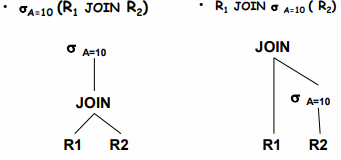
\includegraphics{images/48.PNG}
\end{center}